\chapter{Exemplo de Uso}
\label{cap:elastic}

\section{E-Lastic}
O E-lastic é um sistema eletrônico que monitora e controla a execução de exercícios físicos realizados com equipamento que impõe sobrecarga à movimentação de segmentos corporais por meio de resistência elástica. Esse produto é resultado do trabalho de mestrado em processamento de sinais da aluna Fernanda Sampaio Teles, que resultou num pedido de patente com número de registro BR 5120130007631.

O produto em desenvolvimento apresenta um aparelho portátil, voltado para o controle de atividades físicas em ambientes fechados ou abertos. Trata-se de um sistema eletrônico embarcado que realiza o processamento digital do sinal originado num sensor de força e associa essas informações com variáveis de espaço e tempo, de forma a gerar informações suficientes para o controle e prescrição de exercícios resistidos. Esse sistema eletrônico permite a acoplagem do implemento elástico para a realização do exercício a ser monitorado, e interfaceia com o usuário por meio de um aplicativo. De forma simplificada, durante o exercício físico, a força aplicada pelo usuário ao elemento elástico é calculada no microcontrolador e enviada juntamente com as demais informações via \textit{Bluetooth} para um dispositivo móvel com o e-lastic \textit{app}, que contém opções de controle para a realização do exercício físico.

O código desenvolvido se encontra disponível em um repositório aberto\footnote{\url{http://gitlab.com/biodyn/biodynapp}} para qualquer desenvolvedor através da plataforma gitlab. Não serão explorados aqui detalhes das funcionalidades do aplicativo e-lastic, apenas como foram pensados alguns de seus componentes internos.

\section{Estado da Arquitetura}

O desenvolvimento foi focado na base da arquitetura, juntamente com a funcionalidade básica do aplicativo. Nesta seção, serão chamados de componentes instanciações dos componentes Android, e de módulos conjunto mais complexo de classes que envolvem um ou mais componentes. Na implementação atual do aplicativo, existem os seguintes componentes e módulos principais:

\begin{itemize}
	\item \textit{BluetoothService} - Responsável pela conexão \textit{bluetooth}, este componente é um \textit{Android Service} que se inicia juntamente com a aplicação e fica à espera de uma solicitação de conexão. Quando o usuário solicita a conexão com o hardware e-lastic, o aplicativo identifica o dispositivo a ser conectado e informa ao \textit{BluetoothService}, que a partir daí é responsável por conectar e manter a conexão, recebendo os dados do microcontrolador presente no hardware e-lastic.
	\item \textit{ExerciseService} - Este módulo reúne a maior parte da lógica de negócio. Ele gerencia qual é o exercício ativo e trata da execução do mesmo, controlando informações de entrada vindas do microcontrolador, bem como mudanças nos exercícios solicitadas pelo usuário.
	\item \textit{BioFeedbackService} - Este módulo é responsável por gerar \textit{biofeedback} para o usuário. Quando o valor de força aplicado é superior ao limite máximo, por exemplo, o exercício informa a esse componente que algum tipo de \textit{feedback} deve ser acionado para informar ao usuário que o limite foi ultrapassado.
	\item \textit{ExerciseActivity} - Representa a tela principal e a própria interação do usuário com os componentes gráficos. Neste trabalho, apenas alguns componentes gráficos temporários estão disponíveis para demonstrar a funcionalidade básica do aplicativo em execução.
\end{itemize} 

A comunicação de todos os componentes e módulos é feita de forma indireta por meio de \textit{intents}. O \textit{intent} tem a função de comunicar componentes independente da aplicação a qual pertencem. Entretanto, neste aplicativo em específico, essa comunicação deve ser feita apenas entre os componentes internos da aplicação, não sendo necessário que esses \textit{intents} entre os componentes internos sejam enviados pelo sistema Android para outros componentes de outras aplicações. Para esse fim, a implementação foi feita utilizado um recurso da API Android chamado \textit{LocalBroadcastManager}, que é responsável por realizar o envio de \textit{broadcast intents} apenas para os componentes internos da aplicação, evitando que os mesmos sejam recebidos em outras aplicações. De forma análoga, os receptores desses \textit{intents} são registrados não diretamente no sistema, mas dentro dessa instância de \textit{LocalBroadcastManager} que é individual da aplicação, registrando-se apenas para receber \textit{intents} enviados dentro da própria aplicação. O uso desse recurso evita a necessidade de criar permissões específicas para cada tipo de \textit{intent} que será utilizado entro da aplicação, e não há perigo de que a aplicação receba \textit{intents} forjados por alguma outra aplicação maliciosa ou mesmo que alguma aplicação maliciosa receba dados que são privados deste aplicativo.

Toda essa comunicação indireta foi reunida em uma classe responsável por gerenciar essas comunicações, a classe \textit{Communicator}. Essa classe reúne todas as \textit{actions} de todos os \textit{intents} que as classes estão preparadas para receber. Basicamente, para saber que informações o \textit{ExerciseService} espera, por exemplo, basta checar as constantes na classe \textit{Communicator.ExerciseServiceActions}. Embora essa classe pareça ter um alto acoplamento devido a sua responsabilidade de comunicar todos os componentes, esse acoplamento é reduzido devido a comunicação indireta que é feita com o uso de \textit{intents}. Basicamente, a classe \textit{Communicator} tem a responsabilidade de enviar mensagens para todos os componentes sem realmente os conhecer. Se um componente for alterado, não há impacto algum dentro dessa classe.

Essa comunicação indireta que é implementada por meio dos \textit{intents} tem a vantagem de deixar os componentes com uma conexão bastante fraca. Quando um componente envia uma mensagem, ele não sabe ao certo quem vai receber, portanto não precisa conhecer o receptor. As mensagens são enviadas via \textit{broadcast}, para todos os componentes, e cada um recebe o que desejar receber. Da mesma forma, os receptores dessas mensagens não sabem quem as mandou, e portanto não há uma associação direta em nenhum dos lados da comunicação. Embora pareça deixar a comunicação confusa e embaralhada, isso permite que troquemos um componente inteiro do projeto com pequeno ou nenhum impacto nos demais componentes. A interface gráfica, por exemplo, recebe mensagens do componente de exercício informando sobre atualizações nos dados. Ela não conhece o exercício em execução e o exercício em execução não conhece quem está mostrando seus dados. Se a interface gráfica fosse inteiramente excluída da aplicação, com pouquíssimos ajustes, relacionados principalmente as mudanças no próprio \textit{AndroidManifest.xml}, seria possível deixar várias outras funcionalidades ainda em funcionamento. Com esse acoplamento reduzido entre os componentes da aplicação, se torna muito mais fácil a manutenção e refatoração desses componentes isoladamente, ou mesmo a substituição completa dos mesmos. Trocar o módulo \textit{bluetooth} por um módulo \textit{wifi}, por exemplo, que recebe esses dados por \textit{socket} de rede em vez de \textit{bluetooth}, não traria quase nenhum impacto a aplicação já em produção, uma vez que esse novo módulo poderia simplesmente enviar mensagens da mesma forma que o \textit{bluetooth} enviava utilizando a classe \textit{Communicator}. Como já explicitado, para os demais módulos não importa quem envie os dados, desde que eles cheguem corretamente. 

\begin{figure}[!htb]
\centering
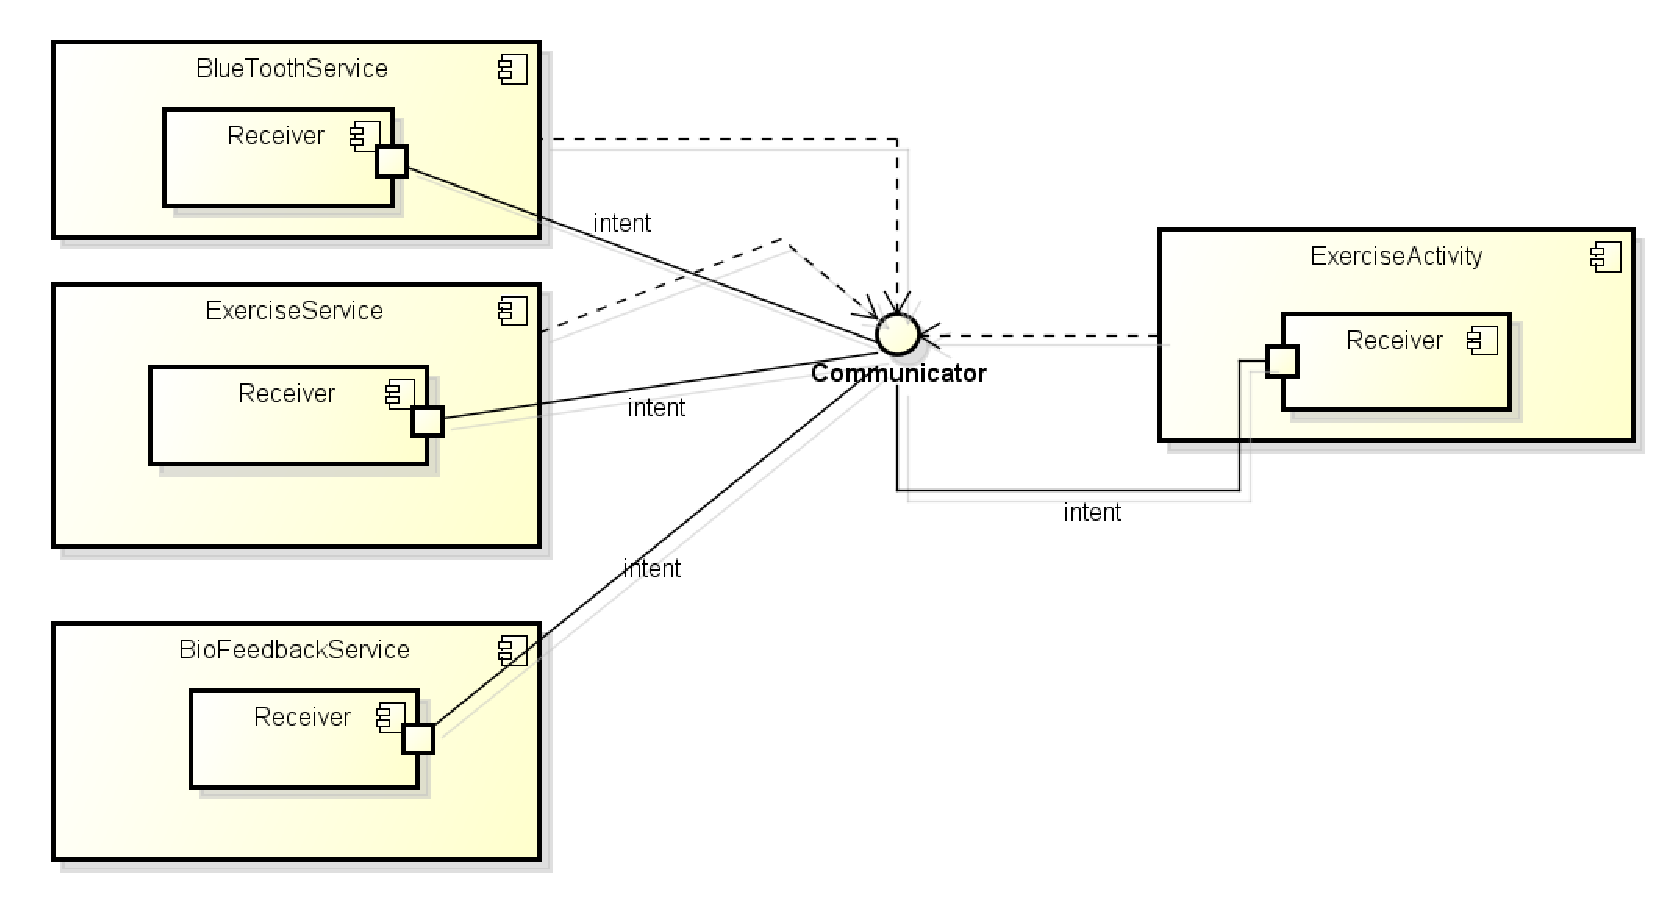
\includegraphics [keepaspectratio=true,scale=0.60]{figuras/diagramaComponentes.eps}
\caption{Componentes e sua comunicação via classe \textit{Communicator}}
\label{diagramaComponentes}
\end{figure}

A única exceção para essa comunicação indireta é a própria inicialização dos componentes. Todos os serviços precisam ser iniciados em algum lugar na aplicação, e o lugar óbvio para o fazer é no início da aplicação. Não tem porque iniciar os componentes enquanto o usuário não abrir a parte gráfica da aplicação, e por esse motivo os serviços são inicializados assim que a \textit{Activity} principal é criada, já que ela é o ponto de entrada da aplicação e-lastic. Muitos componentes podem ser o ponto de entrada em um aplicativo Android, mas neste caso específico a melhor escolha é a própria interface gráfica, representada pela \textit{Activity}. Desse modo a \textit{Activity} conhece os serviços a serem inicializados, porém não conhece seu comportamento e nem mesmo sua responsabilidade.

Essa comunicação por meio do \textit{LocalBroadcastManager} funciona de maneira semelhante ao que vemos no padrão observador de orientação a objetos. Todos os ``eventos'' ou ``mensagens'' gerados em um componente/módulo são informados ao objeto exclusivo ao contexto do aplicativo, que por sua vez os entrega a quem se inscreveu para obtê-los. Uma diferença básica em relação a essa comparação é que no padrão observador, a interface gráfica geralmente conhece a classe de modelo na qual se inscreve para receber atualizações, e portanto existe uma relação unilateral fraca entre os objetos. Da forma implementada neste trabalho, cada objeto apenas conhece as mensagens que quer receber e como elas são formatadas mas não o componente que as envia, deixando as classes mais desacopladas. Entretanto, o resultado de uma análise de fator de acoplamento pode indicar um valor não tão pequeno devido a utilização da classe \textit{Communicator} pelos demais componentes. Nessa arquitetura, é uma classe com alto acoplamento unilateral, pois, embora ela não conheça os componentes que receberão as mensagens, a maioria dos componentes a conhecem e a utilizam como ``mensageiro''. 

A Figura\ref{diagramaComponentes} é um diagrama de componentes que representa de forma gráfica a ideia básica da comunicação entre os componentes da aplicação e-lastic.

\begin{figure}[!htb]
\centering
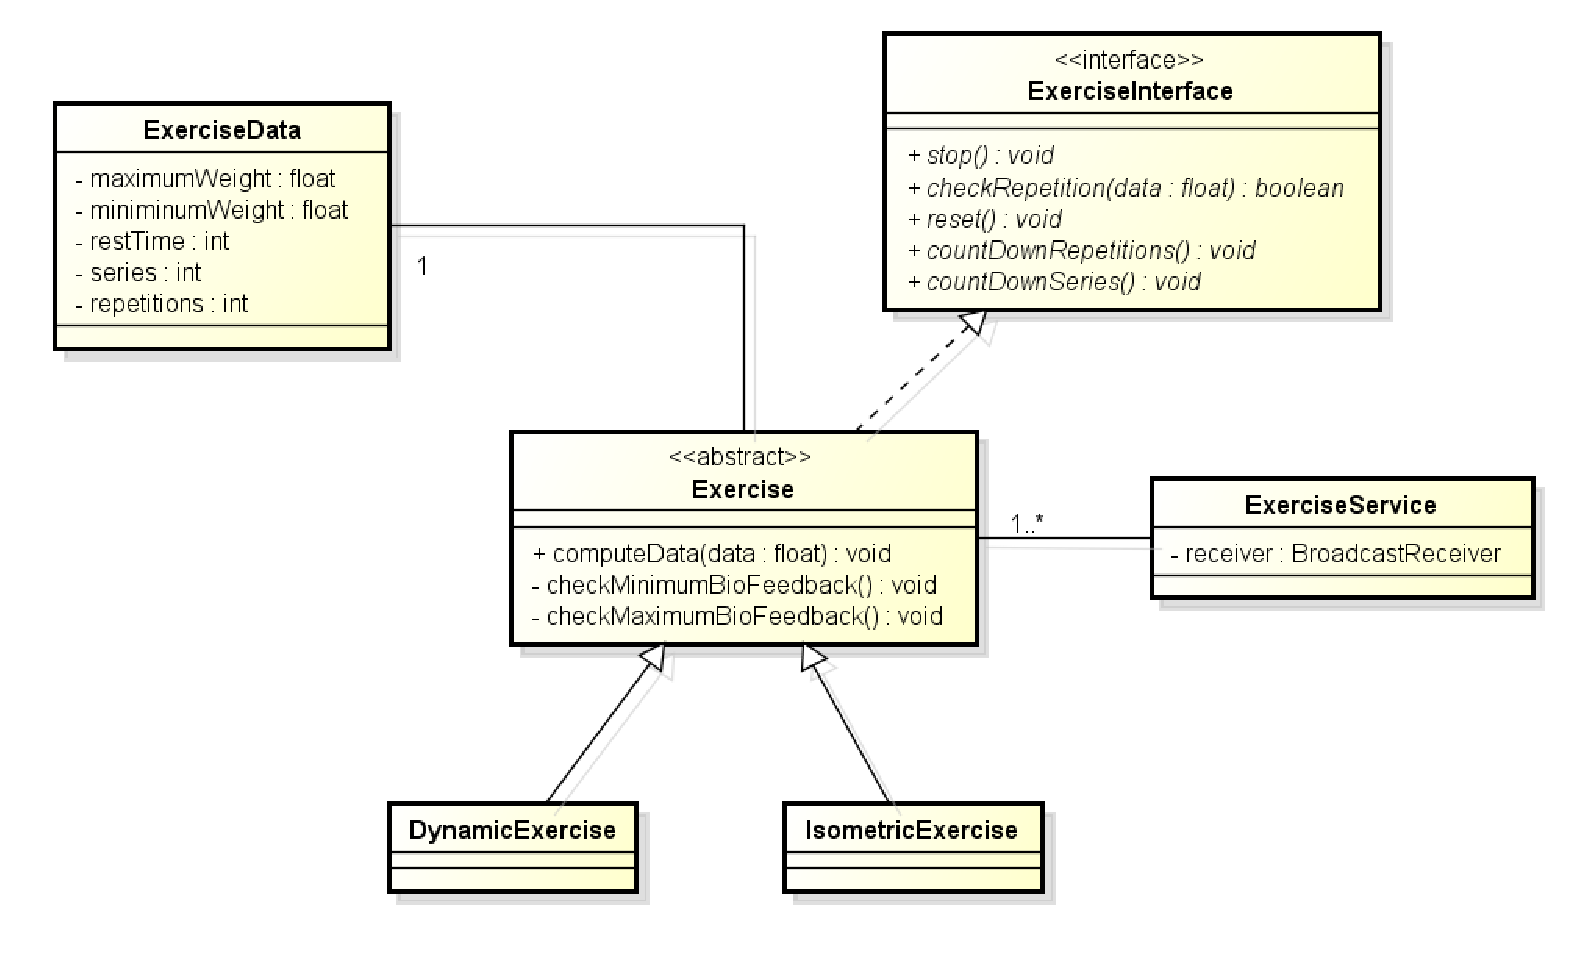
\includegraphics [keepaspectratio=true,scale=0.60]{figuras/diagramaExercicios.eps}
\caption{Principais classes dentro do módulo de exercício e suas relações}
\label{diagramaExercicios}
\end{figure}

Embora representado no diagrama de componentes como uma caixa apenas (\textit{ExerciseService}), o módulo de exercício contém a lógica da comunicação do componente via \textit{Communicator} e o gerenciamento do exercício em execução. É utilizada a generalização para que o \textit{service} tenha o mesmo comportamento independente do exercício em execução, e portanto as manipulações do exercício são feitas em cima de um objeto do tipo \textit{Exercise}, que é uma classe abstrata. A Figura~\ref{diagramaExercicios} contém um diagrama de classes para demonstrar a estrutura básica desse módulo.

\begin{figure}[!htb]
\centering
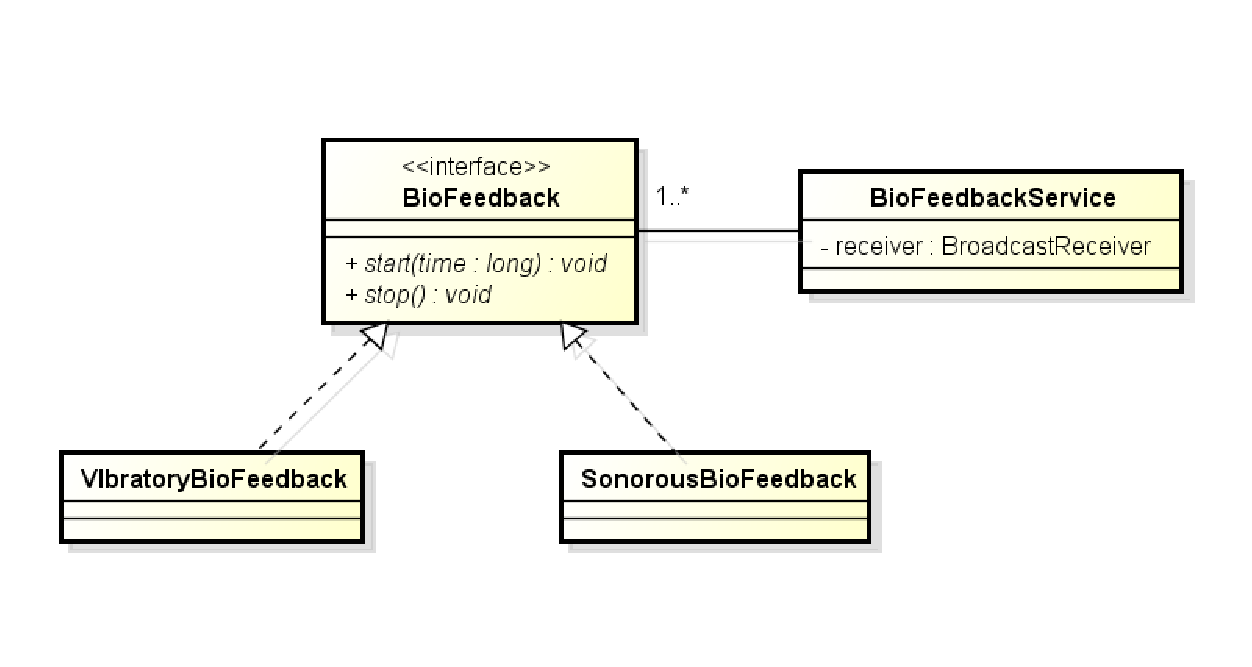
\includegraphics [keepaspectratio=true,scale=0.60]{figuras/diagramaBioFeedback.eps}
\caption{Principais classes dentro do módulo de \textit{biofeedback} e suas relações}
\label{diagramaBioFeedback}
\end{figure}

As classes internas do módulo de \textit{biofeedback} podem ser vistas na Figura~\ref{diagramaBioFeedback}. Também é utilizada uma generalização dos tipos de \textit{biofeedback} com a interface \textit{BioFeedback}, que deve ser implementada para criar um novo tipo de \textit{biofeedback}. Da mesma forma que o módulo de exercício, aqui também existe um \textit{service} que fica em segundo plano a espera de uma requisição de execução de \textit{biofeedback}. Em suma, ele fica em \textit{standby} até que algum pedaço da aplicação solicite que ele ative algum dos seus tipos de \textit{feedback}. Reunir essa função em um módulo específico da aplicação faz com que se possa ter controle de quais tipos de \textit{biofeedback} podem ser utilizados, e eles tem um acesso padrão independente do tipo, com a utilização do \textit{Communicator} e \textit{flags} que identificam que tipos de \textit{biofeedback} ativar. Tocar um som e vibrar o celular são feitos de formas completamente diferentes, e só a própria classe precisa saber como o fazer, sendo que o \textit{service} só conhece a interface de início e término e para ela não importa sua implementação. Com a implementação dessa forma, basta uma adição de uma linha de código no mapa de \textit{biofeedbacks} e a adição de uma \textit{flag}, além da implementação do novo \textit{biofeedback}, para que um novo tipo de \textit{biofeedback} esteja pronto para ser utilizado.

\section{Cálculo de distância aplicado ao E-lastic}
%TODO rever
A arquitetura básica do e-lastic foi submetida a uma coleta de métricas assim como os demais aplicativos do sistema, como apresentado no Capítulo~\ref{cap:analise_exploratoria}. O Score proposto neste trabalho foi aplicado na base arquitetural do aplicativo e-lastic com base nessas métricas coletadas.

\begin{table}[!htb]
\centering
\scalefont{.9}
\begin{tabular}{|l|l|l|l|}
\hline
métrica&75\%&90\%&95\%\\
\hline
accm&1.8&2.33&3.63\\
\hline
amloc&9.97&20.4&23.27\\
\hline
nom&3&5.9&10\\
\hline
noc&0&0&0.95\\
\hline
dit&1&1&1\\
\hline
lcom4&2&3&3.95\\
\hline
acc&0&2.9&4\\
\hline
rfc&10.75&18.8&50.9\\
\hline
\end{tabular}

\caption{Percentis 75, 90 e 95 para as métricas analisadas no aplicativo e-lastic}
\label{tab:biodyn_percentis}
\end{table}

Tomando como referência os intervalos aqui definidos e reunidos na Tabela~\ref{tab:final_table_android}, o aplicativo e-lastic apresenta valores teóricos melhores que os do sistema em todas as métricas, como mostra a Tabela~\ref{tab:biodyn_percentis}. O cálculo resultou em um score de -82, menor que a grande maioria dos aplicativos do sistema, refletindo os ótimos resultados que a Tabela~\ref{tab:biodyn_percentis} apresenta. Em suma, o resultado da análise de métricas classifica o aplicativo e-lastic como tendo uma boa qualidade de código.

%TODO reformular parágrafo de acordo com a reormulação da descrição da hipótese
Os resultados encontrados dão subsídio para afirmar que a hipótese 4 (H4) definida no Capítulo~\ref{cap:metodologia} é verdadeira, isto é, as decisões tomadas ao longo do desenvolvimento do aplicativo com base em padrões de projeto estão relacionadas às decisões tomadas com base em métricas, uma vez que decisões tomadas com este propósito tentariam levar os valores para os menores possíveis, tentando alcançar valores em intervalos ótimos, como os que foram encontrados no aplicativo parcial desenvolvido.
